\documentclass[notheorems,handout]{beamer}
\usefonttheme{serif}
\renewcommand{\rmdefault}{zpltlf} % roman font in math mode
\usepackage{amsthm}
\usepackage[bigdelims,varg]{newpxmath}
\usepackage[bb=px,cal=euler,scr=rsfso]{mathalfa}
\usepackage{bm}
\usepackage[no-math]{fontspec}
\setmainfont{TeXGyrePagellaX}
\usepackage[noindent,UTF8]{ctex} % important to load ctex first

\setlength{\parindent}{0em}
\renewcommand{\baselinestretch}{1.25}

\setbeamertemplate{headline}{
\vspace{3pt}
\footnotesize\kaishu
\parbox[b][1.2em][b]{0.47\paperwidth}{\hfill\color{blue} \insertsection \hspace{1em}}
\hfill
\parbox[b][1.2em][b]{0.47\paperwidth}{\hspace{1em}\color{magenta} \insertsubsection \hfill}
}
\setbeamertemplate{footline}{
\footnotesize\kaishu\color[gray]{0.4}
\parbox[b][1.2em][b]{0.2\paperwidth}{\hspace{1em}\insertshortauthor ·\insertshortinstitute \hfill}
\hfill
\parbox[b][1.2em][b]{0.5\paperwidth}{\centering\insertshorttitle}
\hfill
\parbox[b][1.2em][b]{0.2\paperwidth}{\hfill 第 \insertframenumber {} / \inserttotalframenumber 页\hspace*{1em}}

\vspace{3pt}
}
\setbeamertemplate{sections/subsections in toc}[ball]
\setbeamertemplate{itemize items}[ball]
\setbeamertemplate{enumerate items}[ball]
\setbeamertemplate{theorems}[ams style]
\setbeamercolor{section in toc}{fg=blue,bg=white}
\setbeamercolor{subsection in toc}{fg=magenta,bg=white}
\setbeamerfont{section in toc}{family=\kaishu}
\setbeamerfont{subsection in toc}{family=\kaishu}
\setbeamerfont{frametitle}{series=\bfseries,size=\large}

\usepackage{threeparttable}
\usepackage{booktabs}
\renewcommand{\tablename}{表}

\newtheoremstyle{mydefstyle}{}{}{\fangsong}{}{\bfseries}{}{ }{}
\theoremstyle{mydefstyle}\newtheorem{definition}{定义}
\theoremstyle{mydefstyle}\newtheorem*{assumption}{假设}
\newtheoremstyle{mythmstyle}{}{}{\kaishu}{}{\bfseries}{}{ }{}
\theoremstyle{mythmstyle}\newtheorem{theorem}{定理}
\theoremstyle{mythmstyle}\newtheorem{proposition}{命题}
\theoremstyle{mythmstyle}\newtheorem{lemma}{引理}
\newtheoremstyle{myrmkstyle}{}{}{\fangsong}{}{\kaishu}{}{ }{}
\theoremstyle{myrmkstyle}\newtheorem*{remark}{注}

\newcommand{\diag}{\mathrm{diag}}
\renewcommand{\d}{\mathrm{d}}
\renewcommand{\L}{\mathscr{L}}
\newcommand{\E}{\mathbb{E}}
\renewcommand{\P}{\mathbb{P}}
\newcommand{\var}{\mathrm{var}}
\newcommand{\cov}{\mathrm{cov}}
\newcommand{\hmu}{\hat{\mu}}
\newcommand{\hsig}{\hat{\sigma}}
\newcommand{\hrho}{\hat{\rho}}
\newcommand{\arrowd}{\stackrel{\mathrm{d}}{\rightarrow}}
\newcommand{\arrowp}{\stackrel{\mathrm{p}}{\rightarrow}}
\newcommand{\arrowm}{\stackrel{\mathrm{m}}{\rightarrow}}
\newcommand{\arrowas}{\stackrel{\mathrm{a.s.}}{\rightarrow}}
\newcommand{\F}{\mathcal{F}}
\newcommand{\V}{\mathcal{V}}
\renewcommand{\C}{\mathbb{C}}
\newcommand{\R}{\mathbb{R}}
\newcommand{\Q}{\mathbb{Q}}
\newcommand{\Z}{\mathbb{Z}}
\newcommand{\N}{\mathbb{N}}
\newcommand{\eps}{\varepsilon}
\renewcommand{\emptyset}{\varnothing}
\renewcommand{\top}{\transp}
\DeclareMathOperator*{\argmax}{\mathrm{argmax}}
\newcommand{\blue}{\color{blue}}
\newcommand{\red}{\color{red}}
\newcommand{\green}{\color{green}}


\begin{document}
\title[模板:概率基础]{
\kaishu \Large \textsc{beamer} 模板\\
\heiti \huge 示例:概率论基础}
\author[刘岩]{\kaishu \Large 刘\hspace{1\ccwd}岩}
\institute[武大金融]{\kaishu \large 武汉大学经管学院金融系}
\vskip1em
\date[2021/9/26]{\kaishu \large 2021 年 9 月 26 日}
\frame[plain]{\titlepage}

\kaishu

\frame{\frametitle{本讲内容}\tableofcontents[hideallsubsections]}

\begin{frame}{符号体系}
\begin{itemize}
\item
数字:$a,b,c$ 或 $\alpha,\beta,\gamma$
\item
数系:实数$\R$,有理数$\Q$,整数$\Z$,自然数$\N$
\item
向量-矩阵:列向量 $\bm{x}$,矩阵 $\bm{X}$,转置 $\bm{x}^{\top},\bm{X}^{\top}$,行列式 $\det\bm{X}$
\item
集合:简单情形时,如 $A,B$;多类符号混用时,如 $\mathcal{A,B}$
\item
集合运算:交 $A\cap B$,并 $A\cup B$,补 $A^c$,空集 $\emptyset$
\item
函数:$f(\cdot),F(\cdot)$ 或 $\Phi(\cdot)$
\item
概率算符:概率$\P$,期望$\E$,方差$\var$,协方差$\cov$
\item
一般算符:如滞后算符 $\L$
\item
数学表达:任意 $\forall$,存在 $\exists$,属于 $\in$,包含于 $\subset$
\end{itemize}
\end{frame}

\section{概率空间}
\frame{\frametitle{本节内容}
\tableofcontents[currentsection,currentsubsection,hideothersubsections]}

\begin{frame}{概率空间:样本空间}
\underline{概率空间} (probability space),即三元组 $(\Omega,\F,\P)$
\begin{enumerate}
\item 
$\Omega$:\underline{样本空间} (sample space),一个集合,其元素为各种可能发生的随机状况
	\begin{itemize}
	\item
	如抛硬币,$\Omega = \{H,T\}$,正面、反面;又如 GDP 增速(百分比),$\Omega = [-100,\infty)$
	\item
	样本空间中的点一般记做 $\omega\in\Omega$,称为\underline{样本点} (sample point)或\underline{随机元} (random point)
	\item
	从经济、金融角度看,$\omega$ 称为\underline{状态} (state),$\Omega$称为\underline{状态空间} (state space)更合适
	\end{itemize}
\end{enumerate}
\end{frame}



\section{1-元随机变量}
\frame{\frametitle{本节内容}
\tableofcontents[currentsection,currentsubsection,hideothersubsections]}
\begin{frame}{随机变量:定义}
给定概率空间 $(\Omega,\F,\P)$
\begin{itemize}
\item
\underline{随机变量} (random variable, r.v.) $X$ 是从 $\Omega$ 到实数的一个函数,$X:\Omega \rightarrow \R\cup \{\pm\infty\}$
	\begin{itemize}
	\item
	$\R\cup\{\pm\infty\}$ 表示随机变量可以取值正负无穷;但后续不考虑
	\item
	抛硬币示例:$\omega = H,T$,定义 $X(H) = 0,X(T) = 1$,则 $X$ 的0-1取值反映正负面
	\item
	GDP增速示例:$\omega \in[-100,\infty)$,定义 $X(\omega) = \omega$,则 $\omega$ 即表示状态又表示GDP增速随机变量的取值
	\end{itemize}
\item
这个函数需要满足\underline{可测} (measurable) 的要求:
$$
\underbrace{\{\omega: X(\omega) \le x\}}_{\text{事件}}\in\F,\quad \forall x\in\R
$$
\item[\kaishu 练习]
上面两个例子满足可测性吗?
\end{itemize}
\end{frame}



\section{多元随机变量}
\frame{\frametitle{本节内容}
\tableofcontents[currentsection,currentsubsection,hideothersubsections]}
\begin{frame}{多元随机变量:联合分布}
给定 $(\Omega,\F,\P)$ 及其上定义的 $n$ 个r.v. $X_1,\ldots,X_n$
\begin{itemize}
\item
多元随机事件:$\{X_1\le x_1,\ldots,X_n \le x_n\}$ 表示 $\{X_1\le x_1\},\ldots,\{X_n\le x_n\}$ $n$ 个事件同时发生,即
$$
\{X_1\le x_1,\ldots,X_n \le x_n\} = \bigcap_{1\le i\le n}\{X_i\le x_i\}\in\F
$$
\item
$\forall x_1,\ldots,x_n\in\R$,$X_1,\ldots,X_n$ 的\underline{联合累积分布函数} (joint CDF) 定义为
$$
F(x_1,\ldots,x_n) = \P(X_1\le x_1,\ldots,X_n \le x_n)
$$
简称为\underline{联合分布} (joint distribution)
\end{itemize}
\end{frame}



\section{独立性}
\frame{\frametitle{本节内容}
\tableofcontents[currentsection,currentsubsection,hideothersubsections]}
\begin{frame}{随机变量独立性:定义}
\begin{itemize}
\item
给定 $(\Omega,\F,\P)$,两个事件 $A,B\in\F$ 若满足 
$$
\P(A\cap B) = \P(A)\P(B)
$$
则称为\underline{独立} (independent) 事件
\item
给定 $(\Omega,\F,\P)$ 上的两个r.v. $X,Y$,若 $\forall x,y\in\R$ 满足
$$
\P(X\le x, Y\le y) = \P(X\le x)\P(Y\le y)
$$
则称两个r.v.相互独立
\item
若 $X,Y$ 相互独立,则其联合分布 $F$ 为两个边缘分布 $F_X,F_Y$ 的乘积
$$
F(x,y) = F_X(x)F_Y(y)
$$
\end{itemize}
\end{frame}

\begin{frame}{CLT:Monte Carlo 模拟示例}
\begin{figure}
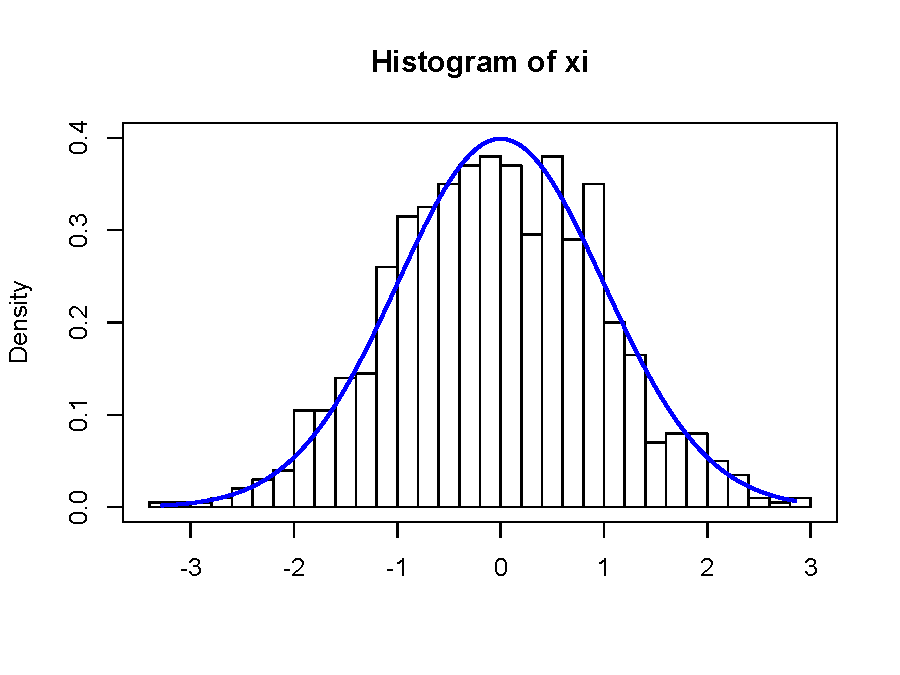
\includegraphics[width=1\textwidth]{CLT.pdf}
\end{figure}
\end{frame}

\end{document}